\documentclass[12pt,letterpaper]{article}

\author{Jordan Bayles}
\title{Homework 2\\
\small ECE 478: Network Security}

%\date{}

%%Usepackage declarations
\usepackage[left=1in,top=1in,right=1in,bottom=1in]{geometry}
\usepackage{lastpage}
\usepackage{sectsty}
\usepackage{slashed}
\usepackage{amsmath}
\usepackage{amsfonts}
\usepackage{latexsym}
% Include for easy import of full pdf pages
\usepackage{pdfpages}
% Include for use of images
\usepackage{graphicx}
% Include for use of [H] placement specifier
\usepackage{float}
% Include for use of \toprule, \midrule, \bottomrule in tabular env.
\usepackage{booktabs}
% Include for setting spacing between lines
\usepackage{setspace}
% Code listing packages
\usepackage{listings}
\usepackage{xcolor}
\usepackage{color}
\usepackage[font=small,format=plain,labelfont=bf,up,textfont=it,up]{caption}
\usepackage[hyphens]{url}

%% Package usages
\sectionfont{\normalsize}
\subsectionfont{\small}

%% New commands
\newcommand{\comment}[1]{}
\newcommand{\field}[1]{\mathbb{#1}} % requires amsfonts
\newcommand{\script}[1]{\mathcal{#1}} % requires amsfonts
\newcommand{\pd}[2]{\frac{\partial#1}{\partial#2}}

%% Access document variables
\makeatletter
\let\thetitle\@title
\let\theauthor\@author
\let\thedate\@date
\makeatother

%% Color Definitions
\definecolor{dkgreen}{rgb}{0,0.6,0}
\definecolor{gray}{rgb}{0.5,0.5,0.5}
\definecolor{mauve}{rgb}{0.58,0,0.82}
\definecolor{lightgrey}{gray}{0.8}
\definecolor{darkgrey}{gray}{1.6}

%% Code Listing Configuration
\DeclareCaptionFormat{listing}{\colorbox{gray}{\parbox{0.987\linewidth}{#1#2#3}}}
\captionsetup[lstlisting]{format=listing, labelfont=white, indention=0pt, textfont=white, margin=0pt, font={bf,footnotesize}, singlelinecheck=false}
\DeclareCaptionFont{white}{\color{white}}
\renewcommand{\lstlistingname}{Code}
\lstset{ %
  %Some lang opts: C++, C, Java, Python, Matlab, TeX, HTML, SQL, Verilog, VHDL, make, ...
  basicstyle=\footnotesize\ttfamily , % the size of the fonts that are used for the code
  numbers=left,                       % where to put the line-numbers
  numberstyle=\scriptsize\color{darkgray}, % the style that is used for the line-numbers
  stepnumber=2,                       % the step between two line-numbers. 
  numbersep=5pt,                      % how far the line-numbers are from the code
  backgroundcolor=\color{white},      % choose the background color. You must add \usepackage{color}
  showspaces=false,                   % show spaces adding particular underscores
  showstringspaces=false,             % underline spaces within strings
  showtabs=false,                     % show tabs within strings adding particular underscores
  frame=tb,                           % adds a frame around the code
  rulesepcolor=\color{gray},          % if not set, the frame-color may be changed on line-breaks within not-black text (e.g. commens (green here))
  tabsize=2,                          % sets default tabsize to 2 spaces
  captionpos=t,                       % sets the caption-position
  breaklines=true,                    % sets automatic line breaking
  breakatwhitespace=false,            % sets if automatic breaks should only happen at whitespace
  title=\lstname,                     % show the filename of files included with \lstinputlisting;
  keywordstyle=\color{blue},          % keyword style
  commentstyle=\color{dkgreen},       % comment style
  stringstyle=\color{mauve},          % string literal style
  escapeinside={\%*}{*)},             % if you want to add a comment within your code
  morekeywords={*,...}                % if you want to add more keywords to the set
  framexbottommargin=5pt,
}

\begin{document}
\begin{flushright}
\theauthor\\
\thedate
\end{flushright}
\begin{center}
\thetitle
\end{center}

\section{Disclaimer}
\emph{This submission reflects my own understanding of the homework and
solutions. All of the ideas are my own, unless I explicitly acknowledge otherwise.}

\section*{1. Database schema}
The database is interfaced with Perl Database Interface Module (DBI), is an
SQLite database, and
contains user credentials in a database called \verb!users!, with at least
two columns entitled \verb!uname! and \verb!pwd!.

\section*{2. SQL Injection vulnerability}
My first step in checking vulnerability was trying a general SQL injection
strategy:

\begin{verbatim}
username: ' or '1'='1' --
password:
\end{verbatim}

This got me into the admin account, since we only check one result from the
database output and presumably it is first alphabetically.

\begin{figure}[H]
	\centering
	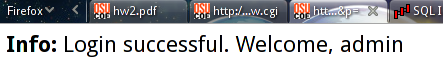
\includegraphics[width=4in]{attempt1.png}
	\caption{First attempt at the database}
\end{figure}

The SQL Injection vulnerability is from when, after checking that the
username field is not empty, the user's input is inserted into
a SQL request verbatim:

\begin{verbatim}
my $sql = "select * from users where uname='$U' and pwd='$P'";
\end{verbatim}

I was really stunned this code was vulnerable to injection, so I spent a while
figuring out why. The exact reason it is vulnerable is because the
username and password are made part of the SQL request before it is compiled.
You should never use place holders with the variable name in Perl for database
requests, but rather use the \verb!?! placeholder and pass in variables
in the \verb!execute! or \verb!do! function\footnote{
\url{http://stackoverflow.com/questions/2300765/how-can-i-protect-against
-sql-injection-attacks-using-perls-dbi}}.

\section*{3. Database in visible output?}
Yes: the username you logged in with is directly shown to you once
you have successfully logged into it.

\section*{4. SQL Injection showing number of columns in users}
First I tried a UNION statement with the \verb!sqlite_master! database
just for fun, and got an error code.

\begin{verbatim}
' or '1'='1' UNION SELECT * from sqlite_master --
\end{verbatim}

\begin{figure}[H]
	\centering
	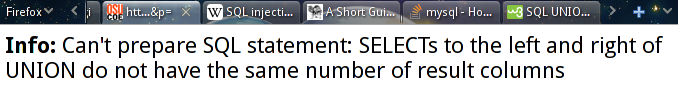
\includegraphics[width=4in]{attempt2.png}
	\caption{Attempt with the sqlite\_master as second database}
\end{figure}

Then I tried something smarter: the \verb!ORDER BY x! argument, which
orders the output based on the $x$-th column. I tried with a value of $x=10$
just to see what would happen:

\begin{verbatim}
' or '1'='1' ORDER BY 10 --
\end{verbatim}

\begin{figure}[H]
	\centering
	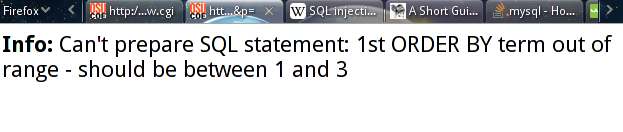
\includegraphics[width=4in]{attempt3.png}
	\caption{Attempt with the ORDER BY argument}
\end{figure}

This told me that the valid column IDs are \verb!1,2,3!, indicating the
users database has \textbf{3 columns}.

\section*{5. SQL injection to find out the name of the table}
We know that the users database will likely contain the name users, so the
easiest way is perhaps this line:
\begin{verbatim}
' UNION SELECT tbl_name,sql,rootpage from sqlite_master where tbl_name LIKE '%user%' --
\end{verbatim}

Which yielded:
\begin{figure}[H]
	\centering
	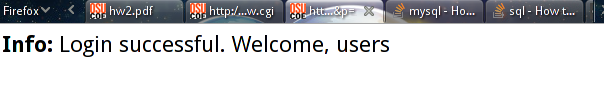
\includegraphics[width=4in]{attempt4.png}
	\caption{Attack finding the name of the users database}
\end{figure}

So we know the name of the database is \verb!users!. The reasons this works
are because (1) the username is not NULL, so the script is executed, (2)
we select three columns from sqlite\_master in order to have the same
number of columns as our user database, and (3) we find all tables that
contain something like "user" in their name, which directly leads to the
\verb~users~ database.

\section*{6. SQL injection to find the SQL schema of users}
The first step here was to see what version of SQLite we were running, just
to double check what our options are:
\begin{verbatim}
' UNION SELECT sqlite_version(), sqlite_version(), sqlite_version();--
\end{verbatim}

This yielded:
\begin{figure}[H]
	\centering
	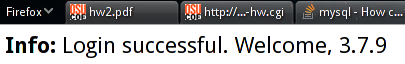
\includegraphics[width=4in]{version.png}
	\caption{Running SQLite version 3.7.9}
\end{figure}

In the end, it was much easier to find this data then I thought it would
be:
\begin{verbatim}
' UNION SELECT sql,null,null FROM sqlite_master WHERE tbl_name = "users"--
\end{verbatim}

Which returns:

\begin{figure}[H]
	\centering
	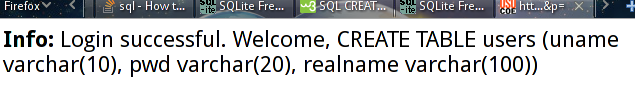
\includegraphics[width=4in]{schema.png}
	\caption{Full schema of table}
\end{figure}

Because the \verb!sql! column is literally the information used to make the
table, all we have to do is get the table information for \verb!users! (null
padded to be the same size as users) from \verb~sqlite_master~.

\section*{7. Attack to find the entire contents of the table}

We know from earlier attempts that the first username is admin, using
the username field query:
\begin{verbatim}
' or '1'='1' --
\end{verbatim}

We can then find the next username by:
\begin{verbatim}
' UNION SELECT MIN(uname), null, null from users where uname > "admin" --
\end{verbatim}

Yielding the username \verb~arnold~

And we can find the rest of the values in the table by the following algorithm:
\begin{verbatim}
user = query(' or '1'='1' --)
results = [user]
while user is not empty:
    user = query(' UNION SELECT MIN(uname), null,
                 null from users where uname > $user --)

    password = query('' UNION SELECT pwd, null,
                     null from users where uname=$user --)

    realname = query('' UNION SELECT realname, null,
                     null from users where uname=$user --)
    add user to results
\end{verbatim}

This algorithm is very simple, we just get the username by doing an alphanumeric
comparison with the last username - effectively iterating through the
usernames - then find the password and realname associated with that
username by filtering for those fields with the username we want.

I decided to - instead of manually iterating - write a python script to do
my dirty work for me. This little beauty uses a linux command line browser
called \verb~twill~ to interface with the webpage, where it can then perform
the queries in the algorithm above, then output them to a table.

\lstinputlisting[language=Python]{sql_injection.py}

Running this script gives the following table.txt file, showing the entire
users table:

\lstinputlisting[language=]{table.txt}

\section*{8. Code patch}
The patch is quick: we just have to patch the vulnerability mentioned in
(2) above, making it so that the SQL code is properly escaped by the
database manager we are using.

\lstinputlisting[language=]{patch}

\section*{9. Works Referenced}
All of the work on this assignment is my own, however I did use references
from the Internet to help with syntax and strategies, so they may have
influenced my work.

\emph{Please let me know if this list is helpful.}

The list of sites referenced:
\begin{itemize}
	\item Python2 Library \\ \url{https://docs.python.org/2/library/}
	\item Twill Documentation \\ \url{http://twill.idyll.org/python-api.html}
	\item Got the idea to use twill from \\ \url{http://stackoverflow.com/questions/5916636/how-to-interact-with-a-webpage-with-python}
	\item SQLite FAQ \\ \url{https://sqlite.org/faq.html}
	\item SQL Injection Powerpoint \\ \url{http://www.cs.rpi.edu/academics/courses/spring10/csci4971/websec2/slides_sqli.pdf}
	\item SQL Column Names in Results \\ \url{http://sqlite.org/c3ref/column_name.html}
	\item W3Schools guide \\ \url{http://www.w3schools.com/sql/sql_create_table.asp}
	\item MySQL table/column names \\ \url{http://websec.wordpress.com/2007/11/17/mysql-table-and-column-names/}
	\item Finding Field Names using SQL Injection \\ \url{http://sqlzoo.net/hack/24table.htm}
	\item SQL Injection Attacks by Example \\ \url{http://www.unixwiz.net/techtips/sql-injection.html}
	\item A Short Guide to DBI \\ \url{http://www.perl.com/pub/1999/10/DBI.html}
	\item SQL Injection: Determining the Number of Columns \\ \url{http://securityreliks.securegossip.com/2011/01/sql-injection-determining-the-number-of-columns/}
	\item How to merge MySQL queries...\\ \url{http://stackoverflow.com/questions/1483690/how-to-merge-mysql-queries-with-different-column-counts}
\end{itemize}
%Sample Code listing
%\lstset{caption={Descriptive Caption Text},label=DescriptiveLabel,language=C}
%\begin{lstlisting}
%!!code!!
%for (int x = 0; x < 5; ++x) {
%	cout << x;
%}
%\end{lstlisting}

% Include a full PDF:
% \includepdf[pages=-]{written_portion.pdf}

% Or for a separate file:
%\lstinputlisting[language=Python]{source_filename.py}

%Sample Figure
% \begin{figure}[H]
%\centering
%\includegraphics[width=4in][scale=1]{file}
%\caption{New caption style}
%\label{fig:}
%\end{figure}

\end{document}
